\documentclass{article}
\usepackage{amsfonts}
\usepackage{amsmath}
\usepackage{listings}
\usepackage{mybigpackage}
\usepackage{graphicx}

\graphicspath{{plots/}}

\begin{document}
	\title{\textbf{Assignment-3}}
	\author{Abheek Ghosh \\ 
		140123047 }
	
	\maketitle
	

\section{Question A, B}

\noindent{Code for R}

\begin{lstlisting}[language=R]
library(mixtools)
rm(list=ls())

expectationMaximization <- function(X, lm, mu1, mu2, sig1, sig2) {
	tol = 10^-5; lim = 100; i = 0

	n = length(X)
	temp1 = dnorm(X, mean = mu1, sd = sig1)
	temp2 = dnorm(X, mean = mu2, sd = sig2)
	M1 = (lm*temp1) / (lm*temp1 + (1-lm)*temp2)
	M2 = 1 - M1
	Q = -1

	repeat {
		lmt = lm; mu1t = mu1; mu2t = mu2; sig1t = sig1; sig2t = sig2;
		i = i + 1
		Q0 = Q

		lm = sum(M1)/n
		mu1 = sum(M1 * X) / sum(M1)
		mu2 = sum(M2 * X) / sum(M2)
		sig1 = sqrt(sum(M1 * (X - mu1)^2 ) / sum(M1))
		sig2 = sqrt(sum(M2 * (X - mu2)^2 ) / sum(M2))

		temp1 = dnorm(X, mean = mu1, sd = sig1)
		temp2 = dnorm(X, mean = mu2, sd = sig2)
		M1 = (lm*temp1) / (lm*temp1 + (1-lm)*temp2)
		M2 = 1 - M1

		Q = sum(M1*log(lm*temp1) + M2*log((1-lm)*temp2))

		if (abs(Q-Q0) < tol || i > lim) {
		# if ((abs(lm-lmt)+abs(mu1t-mu1)+abs(mu2t-mu2)+abs(sig1t-sig1)+abs(sig2t-sig2) < tol)) {
			# print(i)
			break
		}
	}

	return (list(lm = lm, mu1 = mu1, mu2 = mu2, sig1 = sig1, sig2 = sig2))
}

n = 200

lm = 0.4
mu1 = mu2 = 0
sig1 = 1
sig2 = 5

temp_U = runif(n)
temp_X1 = rnorm(n, mean = mu1, sd = sig1)
temp_X2 = rnorm(n, mean = mu2, sd = sig2)

X = temp_X1*(temp_U <= 0.4) + temp_X2*(temp_U > 0.4)

print("From manual implementation of EM")
param = expectationMaximization(X, 0.5, 0, 0, 1, 10);
print( sprintf("lambda = %f, mu1 = %f, mu2 = %f, sig1 = %f, sig2 = %f", 
	param$lm, param$mu1, param$mu2, param$sig1, param$sig2))

print("From built in function normalmixEM")
param = normalmixEM(X)
print( sprintf("lambda = %f, mu1 = %f, mu2 = %f, sig1 = %f, sig2 = %f", 
	param$lambda[1], param$mu[1], param$mu[2], param$sigma[1], param$sigma[2]))
\end{lstlisting}

From manual implementation of EM\\
lambda = 0.399748, mu1 = -0.078376, mu2 = -0.745167, sig1 = 1.316884, sig2 = 5.610553

From built in function normalmixEM\\
lambda = 0.399763, mu1 = -0.078362, mu2 = -0.745193, sig1 = 1.316937, sig2 = 5.610606

We can see that the parameters found by EM algorithm are very close to the actual parameters. Both the EM implementations: manual and built-in give the same output.
\pagebreak

\section{Part C}

\noindent{Code for R}

\begin{lstlisting}[language=R]
rm(list = ls())

n = 100
X = rnorm(n, mean = 0, sd = sqrt(5))
sum_X2 = sum(X^2)

prior <- function (sig2) {
return ((sig2^-3.5) * exp(-1/(2*sig2)))
}

likelihood <- function (sig) {
return (exp(-sum_X2/(2*sig^2)) / (sqrt(2*pi)*sig)^n)
}

posteriorDensity <- function (sig) {
return (likelihood(sig)*prior(sig^2))
}

# Getting the Gamma distribution
k = 1/integrate(posteriorDensity, 0, Inf)$value
t = seq(0, 5, length=1000)
dens = k*posteriorDensity(t)

png("posteriorDensity.png")
plot(t, dens, xlab="x", ylab="Density", type='l')
title("Density of Posterior Inverse-Gamma distribution")
dev.off()

# Bayes Estimate
bayesEstimate <- function (t) {
return (t*k*posteriorDensity(t))
}

be = integrate(bayesEstimate, 0, Inf)$value
print(sprintf("Bayes estimate = %f", be))

# MAP estimator
map = optimize(posteriorDensity, interval=c(0, 30), maximum=TRUE)$maximum
print(sprintf("MAP estimate = %f", map))
\end{lstlisting}

\pagebreak
\textbf{Posterior has Inverse Gamma distribution}

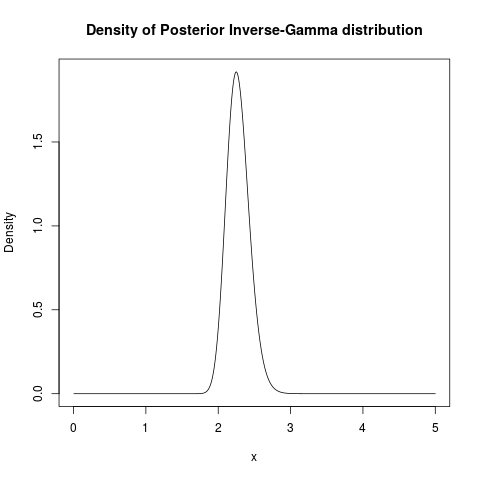
\includegraphics{posteriorDensity.png}
\pagebreak

Given, prior:
\[
p(\sigma^2) \propto (\sigma^2)^{-\frac{5}{2} - 1} \exp(-\frac{1}{2\sigma^2})
\]

Likelihood:
\[
f(X | \sigma) = \frac{1}{(\sqrt{2\pi}\sigma)^n} \exp(\frac{-\sum_{i=1}^{n}x_i^2}{2\sigma^2})
\]
where $n$ is the number of samples $X$. From the above statements we get posterior distribution:
\[
p(\sigma^2|X) \propto f(X | \sigma)\ p(\sigma^2) \propto (\sigma^2)^{-\frac{n}{2}-\frac{5}{2} - 1} \exp(\frac{-1-\sum_{i=1}^{n}x_i^2}{2\sigma^2})
\]
The above equation resembles that on Inverse-Gamma distribution with parameters $\alpha$ and $\beta$, where
\[
\alpha = \frac{5}{2} + \frac{n}{2}
\]\[
\beta = \frac{-1-\sum_{i=1}^{n}x_i^2}{2}
\]\[
p(\sigma^2|X) \propto (\sigma^2)^{-\alpha - 1} \exp(\frac{-\beta}{\sigma^2})
\]

The graph also resembles the inverse gamma distribution with the above mentioned parameters.

Estimated parameters are: \\
Bayes estimate = 2.144515\\
MAP estimate = 2.167212

\end{document}

